\documentclass[12pt]{article}
\usepackage[polish]{babel}
\usepackage[T1]{fontenc}
\usepackage[utf8]{inputenc}
\usepackage{float}
\usepackage{graphicx}

\title{\huge\textbf{System zarządzania partią polityczną -- dokumentacja projektu}}
\author{\Large Jakub Grobelny}
\date{\today}

\begin{document}

\maketitle

\section{Diagram E-R}

\begin{figure}[H]
    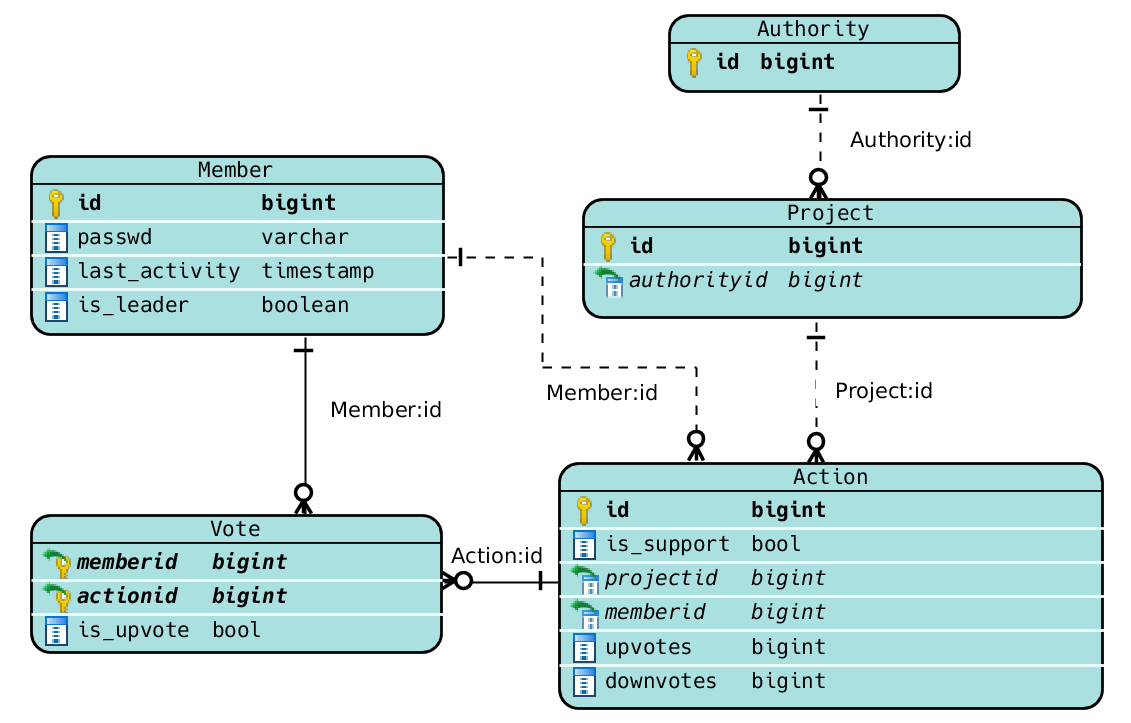
\includegraphics[scale=0.42]{schema-final.png}
\label{figure:er}
\end{figure}

\section{Opis tabel}

\begin{itemize}
    \item{Tabela \textit{Authority} zawiera spis wszystkich organów władzy
          (przechowywane są jedynie ich identyfikatory.)}
    \item{Tabela \textit{Member} zawiera dane wszystkich członków partii.}
    \begin{itemize}
        \item{\textit{id} -- identyfikator członka.}
        \item{\textit{passwd\char`_hash} -- zahaszowane hasło członka.}
        \item{\textit{last\char`_activity} -- czas ostatniej aktywności członka
              używany w celu stwierdzenia, czy jego konto powinno być zamrożone.}
        \item{\textit{is\char`_leader} -- wartość boolowska prawdziwa jeżeli
              dany członek jest liderem partii. W przeciwnym razie fałsz.}
    \end{itemize}
    \item{Tabela \textit{Project} zawiera wszystkie projekty organizowane
          przez organy władzy.}
    \begin{itemize}
        \item{\textit{id} -- identyfikator projektu.}
        \item{\textit{autorityid} -- identyfikator organu władzy organizującego
              dany projekt. Klucz obcy.}
    \end{itemize}
    \item{Tabela \textit{Action} zawiera wszystkie akcje stworzone przez członków
          partii.}
    \begin{itemize}
        \item{\textit{id} -- identyfikator akcji}
        \item{\textit{is\char`_support} -- wartość boolowska prawdziwa, 
              gdy dana akcja popiera projekt organu władzy. 
              Fałszywa, gdy akcja jest protestem}
        \item{\textit{projectid} -- identyfikator projektu, którego dotyczy 
              akcja. Klucz obcy.}
        \item{\textit{memberid} -- identyfikator członka, który utworzył akcję.
              Klucz obcy.}
        \item{\textit{upvotes} -- liczba wszystkich głosów za daną akcję. Pomaga
              w szybkim wyszukiwaniu \textit{trolli}.}
        \item{\textit{downvotes} -- liczba wszystkich głosów przeciw danej akcji. 
              Pomaga w szybkim wyszukiwaniu \textit{trolli}.}
    \end{itemize}
    \item{Tabela \textit{Vote} zawiera spis wszystkich głosów za i przeciw, 
          które zostały oddane na akcje przez członków partii.}
    \begin{itemize}
        \item{\textit{membeid} -- identyfikator członka, który oddał dany głos.
              Klucz obcy.}
        \item{\textit{actionid} -- identyfikator akcji, na którą oddany został
              dany głos. Klucz obcy.}
        \item{\textit{is\char`_upvote} -- wartość boolowska prawdziwa, gdy dany
              głos jest głosem \textit{za}. Fałsz gdy głos jest \textit{przeciw}.}
    \end{itemize}
\end{itemize}

\section{Użytkownicy}

\begin{itemize}
    \item{\textbf{init}} -- użytkownik mający uprawnienia potrzebne do
          wstępnego zainicjowania bazy danych. Powinien móc tworzyć tabele
          (\texttt{CREATE}), wstawiać do nich wartości (\texttt{INSERT})
          oraz nadawać uprawnienia innym użytkownikom (\texttt{GRANT}) aby
          móc utworzyć użytkownika \textbf{app} (\texttt{CREATE USER}).
    \item{\textbf{app}} -- użytkownik mogący odczytywać i modyfikować 
          zawartości wszystkich tabel (\texttt{SELECT, UPDATE, INSERT}) ale 
          niemogący modyfikować schematu bazy danych.
\end{itemize}

\section{Sposób implementacji funkcji API}

Uwaga: ze względu na to, że identyfikatory powinny być globalnie unikatowe, to
każda funkcja tworząca nowe krotki powinna również sprawdzać, czy dany identyfikator
nie pojawił się już dotychczas w którejkolwiek z tabel.

Dodatkowo wszystkie działania wykonywane przez członków powodują, że ich atrybut
\textit{last\char`_activity} zostaje zaktualizowany, jeżeli nie zostali jeszcze
zamrożeni. Funkcje powinny również wcześniej sprawdzać, czy członek wykonujący 
jakieś działanie nie jest zamrożony -- jeżeli jest, to zwracany będzie błąd.

Jeżeli członek nie istnieje, to zostanie utworzony poprzez dodanie odpowiedniej
krotki do tabeli \textit{Member}.

Jeżeli nie istnieje jakiś projekt bądź organ władzy wspomniany w argumentach którejś
z funkcji, to wówczas również powinien zostać dodany do bazy danych.

\begin{itemize}
    \item{\texttt{open} -- w trybie \texttt{init} funkcja \texttt{open} utworzy
          wszystkie tabele opisane powyżej oraz stworzy użytownika \textbf{app}.
          Przy kolejnych uruchomieniach utworzona zostanie sesja dla podanego
          użytkownika}
    \item{\texttt{leader} -- funkcja wstawi do tabeli \textit{Member} nowego
          członka, którego atrybut \textit{is\char`_leader} zostanie ustawiony
          na prawdę.}
    \item{\texttt{support} -- funkcja doda odpowiednią tabeli \textit{Actions},
          której atrybut \textit{is\char`_support} przyjmie wartość prawda.}
    \item{\texttt{protest} -- funkcja analogiczna do \texttt{support}, ale w jej
          przypadku atrybut \textit{is\char`_support} ustawiony zostanie na fałsz.}
    \item{\texttt{upvote} -- funkcja doda nową krotkę do tabeli \textit{Vote} pod warunkiem,
          że dany członek nie głosował jeszcze na daną akcję. Atrybut \textit{is\char`_upvote}
          przyjmie wartość fałsz. Dodatkowo dla tej akcji zwiększona zostanie
          wartość \textit{upvotes} w tabeli \textit{Action}}.
    \item{\texttt{downvote} -- funkcja analogiczna do \texttt{upvote} ale ustawiająca
          wartość atrybutu \textit{is\char`_upvote} na fałsz i zwiększająca atrybut
          \textit{downvotes} zamiast \textit{upvotes} w tabeli \textit{Action}}.
    \item{\texttt{actions} -- funkcja sprawdzi, czy członek wywołujący funkcję
          jest liderem, a następnie wykona odpowiednie zapytanie w celu pozyskania
          danych z tabeli \textit{Action}, które zostaną odpowiednio przefiltrowane
          na podstawie podanych argumentów.}
    \item{\texttt{projects} -- funkcja analogiczna do \texttt{actions} ale
          zapytanie dotyczyć będzie tabeli \textit{Project}.}
    \item{\texttt{votes} -- funkcja sprawdzi, czy członek wywołujący funkcję jest
          liderem a następnie wykona zapytanie, które najpierw zliczy liczbę
          głosów każdego typu użytkowników w tabeli \textit{Vote} a potem
          doda do wyników pozostałych użytkowników, którzy nie oddali być może 
          żadnych głosów.}
    \item{\texttt{trolls} -- funkcja użyje wartości atrybutów \textit{upvotes} i 
          \textit{downvotes} z tabeli \textit{Action} żeby szybko obliczyć bilans
          głosów dla każdej akcji, a następnie pogrupuje akcje według członków,
          którzy je inicjowali, obliczy sumaryczne bilanse głosów i wykluczy
          z wyniku tych członków, dla których ów bilans był pozytywny.}
\end{itemize}

API zostanie zaimplementowane we jęzku \textit{Haskell} przy użyciu biblioteki
\texttt{postgresql-simple}.


\section{Sposób uruchomienia aplikacji}

Przed uruchomieniem programu należy zainstalować \texttt{ghc} oraz 
\texttt{cabal-install}.
Aby skompilować aplikację należy albo uruchomić skrypt \texttt{build.sh} albo
wykonać następujące polecenia:
\begin{itemize}
    \item{\texttt{cabal update}}
    \item{\texttt{cabal sandbox init}}
    \item{\texttt{cabal install ----only-dependencies}}
    \item{\texttt{cabal build}}
\end{itemize}

Skompilowany plik wykonywalny pojawi się w folderze projektu w katalogu 
\texttt{dist/build/databases-project}, i będzie miał nazwę \texttt{databases-project}.

Dodatkowo w głównym folderze projektu po skompilowaniu znajdować będzie się skrót
\texttt{exe} do wygodniejszego uruchamiania programu.

Aby usunąć pliki powstałe po kompilacji należy uruchomić skrypt \texttt{clean.sh}.


\end{document}
